\documentclass[letterpaper,10pt,conference]{ieeeconf}
\IEEEoverridecommandlockouts
\overrideIEEEmargins

\usepackage{amsmath,amssymb,bm}
\usepackage{booktabs}
\usepackage{tabularx}
\usepackage{graphicx}
\usepackage{multirow}
\usepackage{url}
\usepackage{cite}
\usepackage[table]{xcolor}
\usepackage{tikz}
\usepackage{balance}
\usetikzlibrary{arrows.meta,positioning,fit}

% Citation/link blue sampled from the CoSAM manuscript (#367DBD).
\definecolor{cosamLinkBlue}{HTML}{367DBD}

% ieeeconf defines an obsolete Natbib compatibility hook.  Removing it before
% loading hyperref restores clickable numerical citations.
\makeatletter
\let\NAT@parse\undefined
\makeatother
\usepackage[
  colorlinks=true,
  linkcolor=cosamLinkBlue,
  citecolor=cosamLinkBlue,
  urlcolor=black
]{hyperref}

\definecolor{todoRed}{RGB}{176,36,36}
\definecolor{inputBlue}{RGB}{225,238,250}
\definecolor{geometryGreen}{RGB}{224,243,231}
\definecolor{routeOrange}{RGB}{253,237,214}
\definecolor{outputPurple}{RGB}{238,229,247}
\definecolor{transportTeal}{HTML}{12857D}
\definecolor{unsupportedPurple}{HTML}{7455A4}
% % =========================
% % Preamble
% % =========================


% Light lavender section color
\definecolor{sectionband}{RGB}{232,232,252}

\newcommand{\todo}[1]{\textcolor{todoRed}{\textbf{[TODO: #1]}}}
\newcommand{\tbd}{\textcolor{todoRed}{--}}
\newcommand{\captioncolorchip}[2]{%
  \mbox{(\raisebox{0.45ex}{\textcolor{#1}{\rule{1.8ex}{0.30ex}}}%
  \hspace{0.35em}\textcolor{#1}{#2})}}
\newcommand{\R}{\mathbb{R}}
\newcommand{\I}{\mathbf{I}}
\newcommand{\D}{\mathbf{D}}
\newcommand{\K}{\mathbf{K}}
\newcommand{\T}{\mathbf{T}}
\newcommand{\M}{\mathcal{M}}
\newcommand{\F}{\mathbf{F}}
\newcommand{\U}{\mathbf{U}}
\newcommand{\n}{\mathbf{n}}
\newcommand{\od}{\mathbin{\odot}}
\newsavebox{\roboticplatformbox}

\title{\LARGE \bf
DistriNVS: Distributional Geometry Transport and Reliability-Guided Completion for Cross-Endoscope Novel View Synthesis
}

\author{Anonymous Authors}

\begin{document}
\maketitle
\thispagestyle{empty}
\pagestyle{empty}

\begin{abstract}

Cross-endoscope novel view synthesis can broaden the visual context available
to surgical robots by reconstructing a target view from synchronized RGB-D
observations acquired by a spatially displaced endoscope. 
The task is challenging because partial field of view overlap leaves target regions unobserved, 
while sparse or erroneous depth makes source support uncertain.
In this work, we propose DistriNVS, a framework
that separates geometry-supported transport from target-only synthesis. A
reliability encoder first estimates source features, depth distributions,
confidence, and surface orientation. Distributional surface splatting then
propagates these estimates through calibrated geometry and quantifies
target view support, depth variance, and collision ambiguity. Guided by this
evidence, a reliability-constrained gate combines a bounded transport expert
with an uncertainty-conditioned Fourier synthesis expert while preserving
supported source content. Extensive experiments on 1392 iMED\_NVS
test pairs show that DistriNVS achieves the best PSNR, SSIM, and H-PSNR
among the compared reconstruction and completion methods. Without target domain
adaptation, it also achieves the best PSNR, SSIM, and LPIPS among the compared
methods on 275 SCARED test pairs. These results establish reliability-guided transport and synthesis fusion as an effective approach to cross-endoscope
novel view synthesis under partial visual overlap.
\textcolor{cosamLinkBlue}{The code will be made publicly available upon publication.}

\end{abstract}

\section{Introduction}
\label{sec:introduction}

Robot-assisted minimally invasive surgery depends on endoscopic vision for
scene perception and instrument guidance
~\cite{wei2026roboticperception}.
Cross-endoscope novel view synthesis reconstructs a target endoscope image from source endoscope RGB-D observations and the desired source-to-target transformation~\cite{wang2026endoe2egs}.
However, partial field-of-view overlap means that the target may observe anatomy absent from the source views (Fig.~\ref{fig:question}).
The task therefore combines two distinct regimes: co-visible anatomy is
observed in the source view and can be transported through calibrated geometry,
whereas target-only regions have no corresponding source observation and
require image synthesis.
A reliable system should
retain source evidence, identify inferred content, and thereby support
robotic perception with a wider field of view, retrospective visualization,
and surgical simulation~\cite{hsieh2026extrags}.
Such uncertainty-aware cross view completion may also support visual state
construction for surgical robot~\cite{he2025surgworld}.

Achieving this separation is difficult because endoscopic depth estimates
are unreliable around specularities, weak texture, depth discontinuities,
instruments, and deforming tissue~\cite{allan2021scared}. Conventional forward
warping represents each valid source pixel by one 3D point; discretized
projection leaves sampling gaps, while multiple points may compete for the same
target pixel. The binary validity mask conflates missing depth, rasterization
holes, depth sorting conflicts, and cross-endoscope disocclusions.
Treating these cases uniformly either degrades observed structure or permits
hallucination where geometric evidence remains trustworthy.

\begin{figure}[t]
\centering
\vspace*{2mm}
\sbox{\roboticplatformbox}{%
  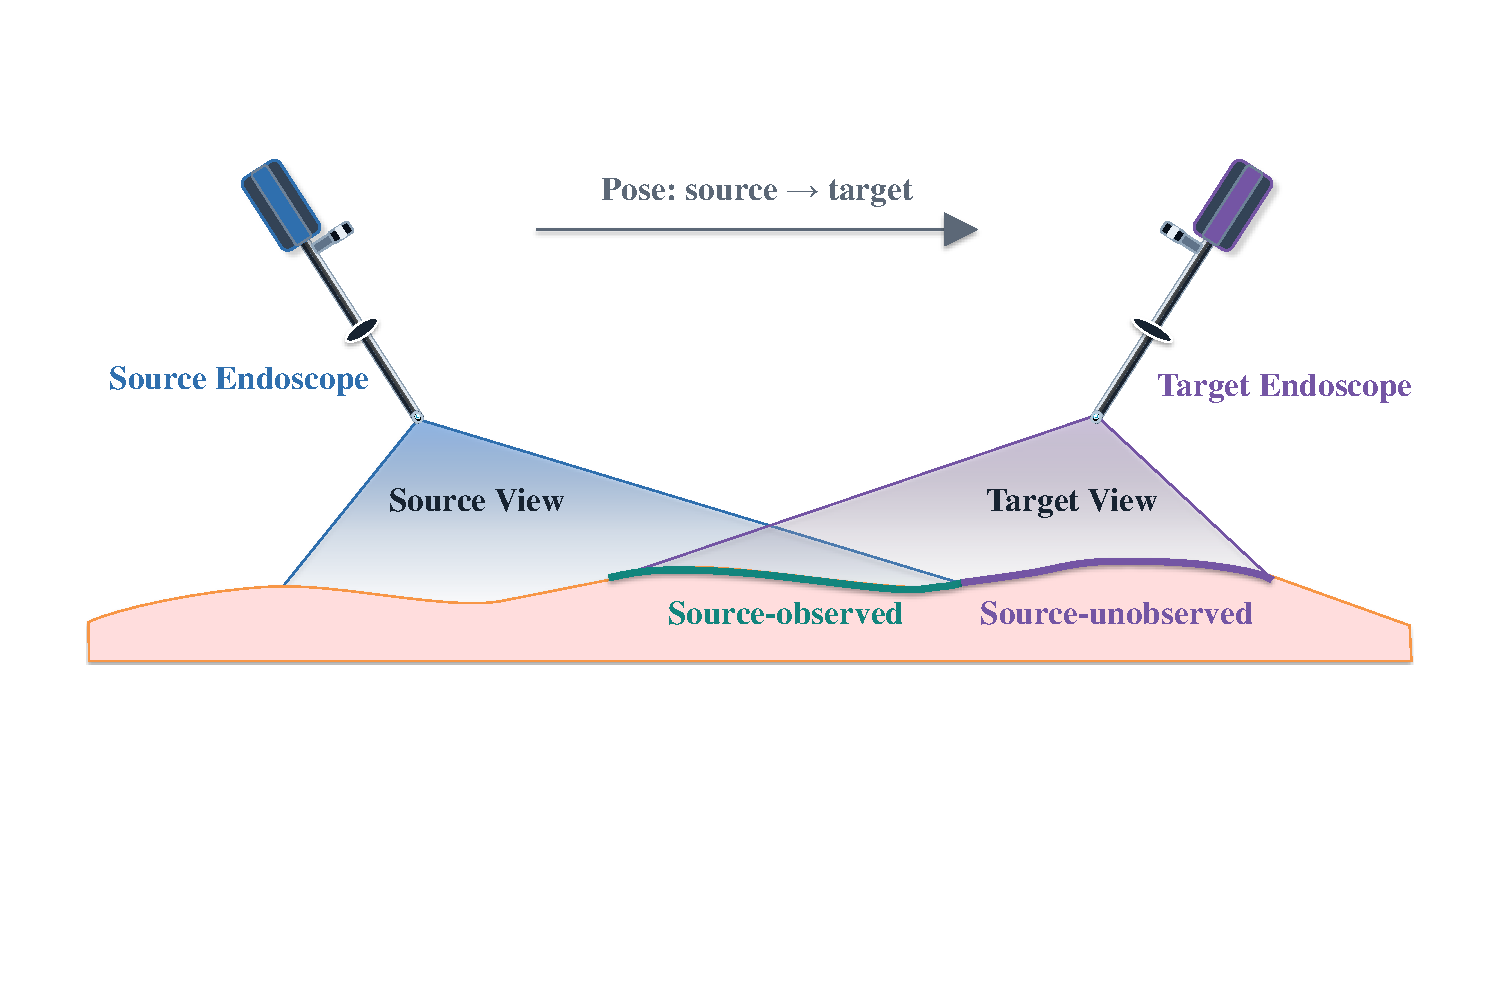
\includegraphics[width=\columnwidth]{figures/distrinvs_teaser/distrinvs_teaser_editable.pdf}%
}
\begin{tikzpicture}
  \clip[rounded corners=0mm]
    (0,0) rectangle
    (\wd\roboticplatformbox,\ht\roboticplatformbox);
  \node[anchor=south west,inner sep=0pt] at (0,0)
    {\usebox{\roboticplatformbox}};
\end{tikzpicture}
\caption{Cross-endoscope novel view synthesis under partial field-of-view
overlap. Given the source to target pose, co-visible anatomy is
source-supported and can be transported through calibrated geometry
\captioncolorchip{transportTeal}{teal}, whereas target-only anatomy lacks source
evidence and needs to be synthesized \captioncolorchip{unsupportedPurple}{purple}.
}
\label{fig:question}
\vspace{-0.4cm}
\end{figure}

Existing methods address parts of this problem. Differentiable point rendering and softmax splatting improve feature transport and collision handling~\cite{niklaus2020softmax}, while reference-guided inpainting combines depth-based alignment with learned completion~\cite{zhao2023geofill}. Large mask inpainting networks provide strong global image priors~\cite{suvorov2022lama}, and endoscopic video completion adds depth, temporal, or stereo cues~\cite{zou2025ssifnet}. Endoscopic neural rendering has advanced sparse view reconstruction and uncertainty modeling~\cite{guo2025ucnerf}. However, the approaches address uncertainty before or after view transformation. Deterministic projection assigns the same reliability to all valid depths, while uncertainty in image space characterizes uncertainty in the target image domain. The propagation of depth uncertainty for each source pixel through a spatially displaced cross-endoscope transform remains less explored.

% Neither approach propagates per-pixel
% depth uncertainty through the cross-endoscope transform and uses the resulting
% visibility statistics to constrain where appearance may be synthesized.



\begin{figure*}[t]
\centering
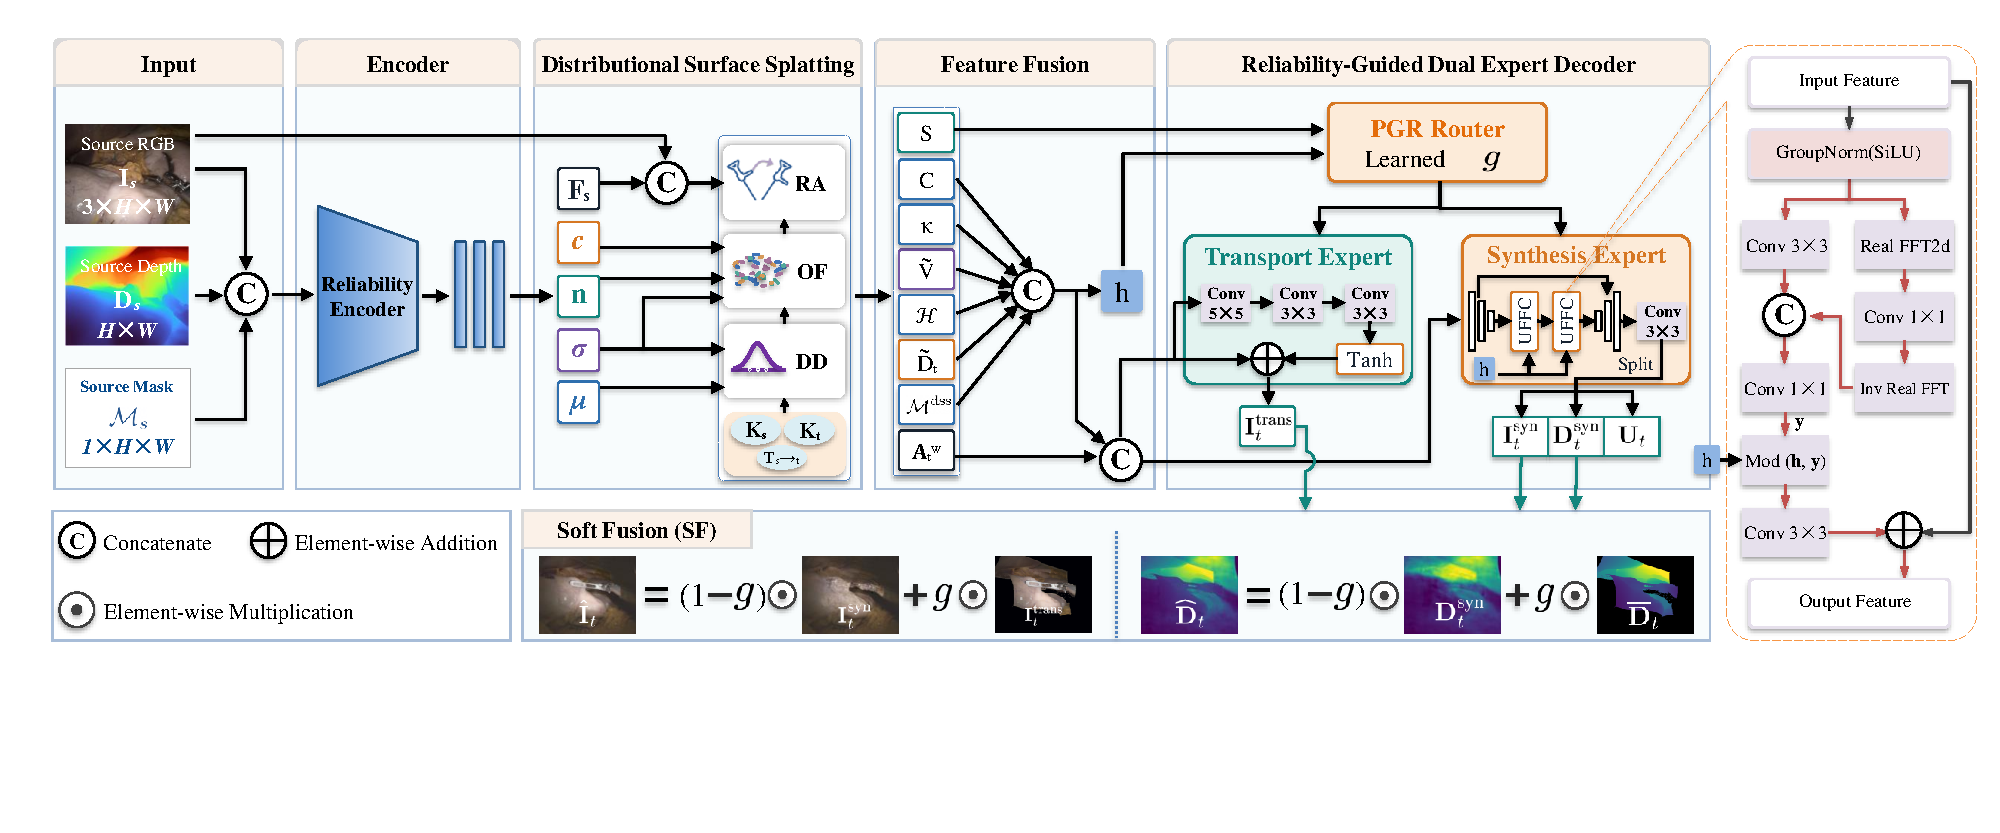
\includegraphics[width=\textwidth]{figures/framework/framework.pdf}
\caption{DistriNVS framework. Encoder outputs $\F_s,c,\n,\sigma,\mu$; DSS
outputs $S,C,\kappa,\widetilde V,\mathcal H,\widetilde D_t,\M^{\rm dss},
\mathbf A_t^w$; and the PGR gate and branch predictions
$g,\I_t^{\rm trans},\I_t^{\rm syn},\D_t^{\rm syn},\U_t$ are detailed in
Secs.~\ref{sec:reliability-encoder}, \ref{sec:dss},
and~\ref{sec:expert-fusion}, respectively. The framework outputs fused target
RGB $\widehat\I_t$, fused target depth $\widehat\D_t$, and target-view risk
$\U_t$. In each UFFC block,
$\operatorname{Mod}(\mathbf h,\mathbf y)$ modulates the fused local Fourier
feature $\mathbf y$ using the resized reliability condition $\mathbf h$.
}
\label{fig:overview}
% \vspace{-0.4cm}
\end{figure*}


% Our central premise is to \emph{transport reliable geometric evidence and
% synthesize only unsupported or geometrically unreliable regions}. 
In this paper, we introduce DistriNVS, a reliability-aware framework
for direct cross-endoscope novel view synthesis. Its distributional surface
splatting (DSS) represents each source depth as a distribution whose bounded
mean and scale, surface normal, and confidence are predicted by a depth
reliability encoder.
DSS projects deterministic depth hypotheses through the
calibrated cross-endoscope transform and aggregates source features using
footprints with soft nearest surface visibility,
yielding target support, depth variance, and collision entropy. These statistics
constrain a soft mixture between bounded residual transport for co-visible
regions and uncertainty-conditioned Fourier completion for unsupported or
ambiguous regions.
% Target-depth and risk prediction plus backward RGB-D
% reprojection constrain this mixture during training.
The paper makes three contributions:
\begin{itemize}
    \item We propose a reliability-aware framework for cross-endoscope novel view 
    synthesis that separates the transport of anatomy observed in the source
    view from the synthesis of content unobserved in the source view.
    \item We introduce DSS, a differentiable renderer that propagates depth
    distributions through calibrated cross-endoscope geometry and exposes
    target support, depth variance, and collision entropy beyond binary validity.
    \item We design a decoder with dual experts that forms a soft mixture of bounded
    residual transport and uncertainty-conditioned Fourier completion under a
    reliability constraint.
\end{itemize}



\section{Related Work}
\label{sec:related}

We summarize image completion, geometry-guided view transport, and
endoscopic neural rendering, with particular attention to how existing
approaches represent missing content, exploit calibrated geometry, and quantify
uncertainty.


\subsection{Image and Endoscopic Video Inpainting}

Generic image inpainting combines mask-aware feature extraction with
broad appearance priors. Partial and gated convolutions prevent
invalid activations from contaminating local features
~\cite{yu2019gated}, whereas LaMa and UFFC use Fourier operations
for global context and MAT restricts attention to valid tokens
~\cite{suvorov2022lama,chu2023uffc,li2022mat}. Recent diffusion models such as
BrushNet and TurboFill incorporate masked image features into pretrained
generators or adapt sampling with few steps for efficient completion
~\cite{ju2024brushnet,xie2025turbofill}. Despite strong appearance priors, these
methods define holes in a fixed image coordinate system and do not describe
geometric provenance. Endoscopic completion adds domain cues: DAEVI combines
spatiotemporal RGB and depth, and SSIFNet fuses flow and stereo temporal
information for instrument occlusions
~\cite{zhang2024daevi,zou2025ssifnet}. Such methods exploit
neighboring frames or views but still restore defects defined in the original
camera coordinates.
Cross-endoscope synthesis instead creates holes through viewpoint transfer, while rasterization gaps or depth conflicts may retain source support. In this paper, the proposed DistriNVS uses calibrated projection statistics to distinguish true disocclusions from rasterization gaps and depth conflicts.

% Cross-endoscope synthesis instead creates holes through
% viewpoint transfer: target-only anatomy is unobserved, while rasterization gaps
% or depth conflicts may retain source support. DistriNVS therefore uses
% calibrated projection statistics to distinguish true disocclusions from
% rasterization gaps and depth conflicts.

\subsection{Geometry-Guided Transport and Completion}

Geometry-guided view synthesis preserves correspondence by transporting source
evidence before generating missing content. SynSin predicts and projects a
feature point cloud, softmax splatting resolves many-to-one mappings with
learned importance, and GeoFill refines depth and pose before reprojection and
inpainting~\cite{wiles2020synsin,niklaus2020softmax,zhao2023geofill}. Recent
feedforward Gaussian renderers use stronger explicit representations. MVSplat
localizes Gaussians with plane-sweep cost volumes, whereas DepthSplat combines
multi-view correspondence with monocular depth priors
~\cite{chen2024mvsplat,xu2025depthsplat}. They reduce the need for optimization
for each scene but
infer a radiance representation from multiple calibrated observations, without
an explicit per-pixel boundary between measured and synthesized appearance.
Generative methods address wider view gaps by synthesizing missing content from reference or geometric cues.
LeftRefill frames synthesis conditioned on a reference as paired canvas
completion, MultiDiff conditions video diffusion on warped depth reference
views, and latent diffusion guided by points uses clouds derived from stereo for
laparoscopic view synthesis
~\cite{cao2024leftrefill,muller2024multidiff,tang2025pointguided}.
These models can synthesize missing regions but do not distinguish whether a target pixel is supported by reliable source geometry. 
In contrast, DistriNVS estimates support from the source view for each target pixel, preserves transported source content in reliable regions, and applies synthesis to unobserved regions.

% These models can
% generate plausible structures in large disocclusions, 
% yet plausibility alone does not reveal which pixels retain geometric support.
% % yet plausibility alone
% % does not reveal which pixels remain geometrically supported. 
% DistriNVS instead
% transports a calibrated source observation with distributional splatting,
% derives support, variance, and collision statistics during rasterization, and
% uses them to constrain soft fusion between transported and synthesized content.







\begin{figure*}[t]
\centering
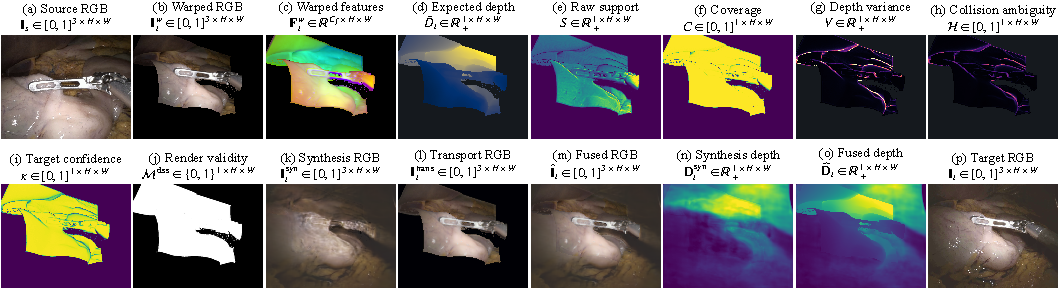
\includegraphics[width=\textwidth]{figures/framework/dss_network_output_grid.pdf}
\caption{DSS evidence and network predictions for a representative iMED\_NVS pair. (a) Source RGB. (b)--(j) Transported attributes and reliability
statistics produced by DSS. (k)--(o) Synthesis, transport, and fused RGB-D
predictions. (p) Target RGB. Scalar maps are
pseudocolored for visualization.}
\label{fig:dss-network-outputs}
\vspace{-0.4cm}
\end{figure*}






\subsection{Endoscopic Novel View Synthesis and Uncertainty}

Endoscopic neural rendering handles nonrigid tissue, illumination, tool occlusions, and sparse camera coverage. EndoNeRF represents
deformation with a neural radiance field, while EndoSurf combines dynamic
modeling with a neural surface~\cite{wang2022endonerf,zha2023endosurf}.
EndoSparse introduces geometric and appearance priors into Gaussian splatting,
and Endo-GSMT uses depth, dense displacement, and motion priors for dynamic
reconstruction~\cite{li2024endosparse,gou2025endogsmt}. GastroNVS further shows
that large viewpoint changes in real gastroscopy amplify geometric artifacts
and illumination mismatch between views~\cite{minai2026gastronvs}. These systems
build persistent scene representations from multiple frames and address
reconstruction fidelity within a captured scene. 
There also exist uncertainty-aware approaches for addressing sparse evidence in endoscopic scenes.
UC-NeRF conditions a
radiance field on multi-view uncertainty, whereas ExtraGS uses uncertainty to
sample virtual cameras and weight pseudo observations refined by diffusion for
extrapolation~\cite{guo2025ucnerf,hsieh2026extrags}.
% Thus, neither uncertainty nor
% generative priors are new to endoscopic rendering.
In contrast, we propagate a distribution for each input depth through the
calibrated cross-endoscope transform and derive target support, depth variance,
and collision entropy from the same rasterization that transports appearance.
% DistriNVS uses these quantities to route completion during unseen-sequence
% inference without target-scene optimization.




\section{Method}
\label{sec:method}

% \subsection{Problem Formulation}

% After resizing, both endoscope views have spatial size $H\times W$; we omit the
% batch dimension throughout. 
DistriNVS receives source RGB
$\I_s$, metric depth
$\D_s\in\R_+^{1\times H\times W}$, validity mask
$\M_s\in\{0,1\}^{1\times H\times W}$, source and target intrinsics
$\K_s,\K_t\in\R^{3\times3}$, and the rigid cross-endoscope transform
$\T_{s\rightarrow t}\in\mathrm{SE}(3)\subset\R^{4\times4}$. The model predicts
target RGB $\widehat\I_t$, depth $\widehat\D_t$, and risk
$\U_t\in[0,1]^{1\times H\times W}$. A reliability encoder first estimates
source features, geometry, and uncertainty. DSS transports these attributes
into the target view and derives expected depth, support, and ambiguity. The
transported attributes and reliability maps condition the transport expert,
synthesis expert, and router. The router produces a reliability-constrained
soft gate that fuses the two expert predictions into the final target RGB-D.
The synthesis head estimates target-view risk.
We denote the reliability encoder, depth-distribution construction,
orientation-aware footprint computation, reliability aggregation, and
expert prediction by $f_{\rm enc}$, $f_{\rm DD}$, $f_{\rm OF}$,
$f_{\rm RA}$, and $f_{\rm exp}$, respectively.
Fig.~\ref{fig:overview} summarizes the pipeline of the proposed method.

\subsection{Reliability Encoder}
\label{sec:reliability-encoder}
The reliability encoder constructs the source geometric representation
for DSS by modeling the reliability of measured and inferred depths.
% It takes source RGB, normalized sparse depth, and its validity mask as input.
A branch at full resolution preserves local boundaries through residual
convolutional blocks, while a branch at quarter resolution captures broader
context using strided convolution. The context features are upsampled using
bilinear interpolation, concatenated with the features from the branch at full
resolution, and fused through a residual connection. A shared prediction head
produces a feature map
$\F_s\in\R^{C_f\times H\times W}$ and raw depth, scale, confidence, and
orientation parameters. These parameters yield depth fields
$\mu,\sigma\in\R_+^{1\times H\times W}$, confidence
$c\in[0,1]^{1\times H\times W}$, and a unit-length orientation proxy
$\n\in\R^{3\times H\times W}$. We denote the complete encoder mapping by
\begin{equation}
 (\F_s,\mu,\sigma,c,\n)
 =f_{\rm enc}(\I_s,\D_s,\M_s).
 \label{eq:reliability-encoder}
\end{equation}

The shared prediction head applies bounded residual corrections to measured
depths and infers missing depths through a \emph{depth completion (DC)}
parameterization. When DC is enabled, both measured and completed depths
participate in DSS, with reduced confidence assigned to completed estimates.
The orientation proxy is learned under the downstream objectives and is used
to adapt the splat footprint. During training, random depth dropout exposes the
encoder to both measured and missing depth patterns, while depth supervision is
retained on the originally valid samples.




\subsection{Distributional Surface Splatting}
\label{sec:dss}
DSS comprises Distributional Depth (DD), Orientation-aware Footprints (OF), and
Reliability Aggregation (RA). DD propagates source depth uncertainty through
the calibrated cross-endoscope transform using deterministic depth hypotheses.
OF adapts each projected footprint to depth uncertainty and surface
orientation. RA aggregates the transported hypotheses and derives reliability
statistics in the target view for downstream routing.

\textbf{Distributional depth (DD).}
Given the predicted mean $\mu$ and scale $\sigma$, DD constructs three depth
hypotheses using fixed offsets $\xi_j\in\{-1,0,1\}$ and normalized Gaussian
weights $a_j$, where $\sum_{j=1}^{3}a_j=1$. The calibrated pinhole operator
$\Pi_{s\rightarrow t}$ back-projects each hypothesis with $\K_s$, applies
$\T_{s\rightarrow t}$, and projects it with $\K_t$. Specifically,
$z_j=\mu+\xi_j\sigma$ and
$(\mathbf X_j,D_j^t)=\Pi_{s\rightarrow t}
(z_j,\K_s,\K_t,\T_{s\rightarrow t})$ for $j\in\{1,2,3\}$.
The complete DD mapping is
\begin{equation}
 \{z_j,a_j,\mathbf X_j,D_j^t\}_{j=1}^{3}
 =f_{\rm DD}(\mu,\sigma,\K_s,\K_t,\T_{s\rightarrow t}),
\label{eq:dd-function}
\end{equation}
where $z_j,D_j^t\in\R_+^{1\times H\times W}$ denote the source depth
hypothesis and its depth in the target frame, respectively, and
$\mathbf X_j\in\R^{2\times H\times W}$ contains
the projected target coordinates~\cite{wiles2020synsin,niklaus2020softmax}.

\textbf{Orientation-aware footprints (OF).}
For each projected hypothesis, OF constructs an elliptical footprint based on
projection sensitivity, predicted depth uncertainty, and surface orientation,
with $\mathbf r_j=b+|\mathbf J_j|\odot\sigma+b_n(1-|n^z|)$.
The complete OF mapping is
\begin{equation}
 \{\mathbf r_j\}_{j=1}^{3}=f_{\rm OF}\!\left(
 \{\mathbf X_j,D_j^t\}_{j=1}^{3},\sigma,\n;b,b_n\right),
\label{eq:of-function}
\end{equation}
where $\mathbf J_j,\mathbf r_j\in\R^{2\times H\times W}$ denote the projection
sensitivity along two axes and footprint radii, respectively, while $b$ and
$b_n$ control the base expansion and the expansion based on orientation. Each hypothesis is
splatted using weights determined by confidence $c$, the hypothesis weight
$a_j$, distance within the elliptical footprint, and soft nearest-surface depth
ordering. Nearest-depth
selection and integer assignment are discrete; the remaining operations are
differentiable.

\textbf{Reliability aggregation (RA).}
RA uses the distributional footprints to transport the concatenated source
attributes $\mathbf A_s=[\I_s,\F_s]\in\R^{(3+C_f)\times H\times W}$. RA
aggregates overlapping hypotheses to produce
$\mathbf A_t^w=[\I_t^w,\F_t^w]\in\R^{(3+C_f)\times H\times W}$, the expected
depth $\bar D_t$, and the conditional depth variance $V$. Raw support is mapped
to bounded coverage $C$ and render validity $\M^{\rm dss}$. Collision ambiguity
$\mathcal H$ is computed from normalized weight entropy and depth dispersion,
discounting benign subpixel overlap. Target confidence $\kappa$ is
derived from $(C,V,\mathcal H)$. The complete aggregation is
\begin{equation}
\begin{aligned}
&(\mathbf A_t^w,\bar D_t,S,V,C,\mathcal H,\kappa,\M^{\rm dss})\\
&\quad=f_{\rm RA}\!\left(
\mathbf A_s,c,\{\mathbf X_j,D_j^t,a_j,\mathbf r_j\}_{j=1}^{3};\tau_z
\right),
\end{aligned}
\label{eq:ra-function}
\end{equation}
where $S$ denotes raw geometric support, $V$ depth variance, $C$ bounded
coverage, $\mathcal H$ collision ambiguity, and $\kappa$ target confidence.
Together, these statistics provide continuous geometric evidence beyond the
binary render validity mask. Fig.~\ref{fig:dss-network-outputs} visualizes these
DSS outputs alongside the downstream network predictions.






\subsection{Reliability-Guided Dual Expert Fusion}
\label{sec:expert-fusion}

\textbf{Physics-guided routing (PGR).}
PGR forms the reliability condition
$\mathbf h=[C,\kappa,\widetilde V,\mathcal H,\widetilde D_t,\M^{\rm dss}]
\in\R^{6\times H\times W}$, where $\widetilde V$ is the normalized form of
$V$ and $\widetilde D_t$ is the normalized form of $\bar D_t$. A synthesis
prior $g^0\in[0,1]^{1\times H\times W}$ derived from physics increases with
decreasing confidence, increasing depth dispersion, and increasing collision ambiguity. For
render-valid pixels, the prior is computed from the weighted reliability terms,
whereas pixels without DSS support are assigned a synthesis prior of one,
yielding $g^0=(1-\M^{\rm dss})+\M^{\rm dss}\odot
[\lambda_\kappa(1-\kappa)+\lambda_V\widetilde V+\lambda_H\mathcal H]$.
Before conversion to logit space, the prior is clipped to
$[\epsilon,1-\epsilon]$ for numerical stability. 
The reliable support mask $\M^{\rm rel}\in\{0,1\}^{1\times H\times W}$,
obtained as $\M^{\rm rel}\leftarrow(S,V,\mathcal H,\M^{\rm dss})$, marks DSS
evidence as reliable when the render is valid, support is sufficient, and depth
variance and collision ambiguity remain below their thresholds. The router
adds a bounded residual $\Delta_\theta(\mathbf h)\in\R^{1\times H\times W}$
to the detached prior logit, where $\operatorname{sg}(\cdot)$ denotes the
stop-gradient operation.
The effective synthesis gate $g\in[0,1]^{1\times H\times W}$ is
\begin{equation}
 g=(1-\M^{\rm rel})\odot\operatorname{sigmoid}\!\left(
 \operatorname{sg}[\operatorname{logit}(g^0)]+\Delta_\theta(\mathbf h)\right).
\label{eq:effective-gate}
\end{equation}

\textbf{Complementary experts.}
We employ a \emph{transport expert} to correct source-supported appearance and
a \emph{synthesis expert} to generate content where geometric evidence is
unreliable. We form the shared expert input by concatenating the transported
content and reliability evidence as $\mathbf X_t=[\mathbf A_t^w,\mathbf h]
\in\R^{(C_f+9)\times H\times W}$. Given $(\mathbf X_t,\I_t^w)$, the transport
expert predicts a bounded RGB correction to $\I_t^w$ while retaining the DSS
expected depth $\bar D_t$. The synthesis expert processes $(\mathbf X_t,\mathbf h)$
with a Fourier U-Net operating at four resolutions and conditioned on
uncertainty~\cite{ronneberger2015unet}. A $5\!\times\!5$ stem first projects
$\mathbf X_t$ to 32 channels. The resulting features are then processed by
three stride-2 encoder stages and three symmetric decoder stages with bilinear
upsampling and skip connections. Each stage contains an uncertainty-conditioned
Fourier convolution (UFFC) block. The block sends normalized features through
a local $3\!\times\!3$ convolution branch and a parallel global Fourier branch.
The Fourier branch applies a 2D real
FFT~\cite{suvorov2022lama} and mixes the concatenated real and imaginary
coefficients using a $1\!\times\!1$ convolution. An inverse real FFT maps the
mixed coefficients back to the spatial domain. A $1\!\times\!1$ convolution
fuses the outputs of the two branches. At every resolution, a learned
affine transform derived from the resized condition tensor $\mathbf h$
modulates the fused features before residual addition. A final
$3\!\times\!3$ head jointly predicts RGB logits, normalized depth, and risk.
The expert outputs are $\I_t^{\rm trans}$, $\I_t^{\rm syn}$,
$\D_t^{\rm syn}$, and $\U_t\in[0,1]^{1\times H\times W}$. We denote the joint
expert mapping by
\begin{equation}
 (\I_t^{\rm trans},\I_t^{\rm syn},\D_t^{\rm syn},\U_t)
 =f_{\rm exp}(\mathbf X_t,\I_t^w,\mathbf h).
\label{eq:expert-function}
\end{equation}

% Unlike mask-conditioned Fourier inpainting networks
% ~\cite{suvorov2022lama,chu2023uffc}, our 
% The local--global design injects
% continuous DSS reliability at every resolution.
% All weights are trained
% jointly within DistriNVS. Risk is trained as an error-scale proxy on unreliable
% regions, not as a calibrated failure probability over the full image.

\textbf{Reliability-constrained output.}
The transport branch retains source evidence while allowing bounded appearance
correction; the synthesis branch supplies content where geometric evidence is
weak. The fused RGB prediction is
\begin{equation}
 \widehat\I_t=(1-g)\odot\I_t^{\rm trans}+g\odot\I_t^{\rm syn}.
\label{eq:expert-fusion-rgb}
\end{equation}

The fused depth prediction is
\begin{equation}
 \widehat\D_t=(1-g)\odot\bar D_t+g\odot\D_t^{\rm syn}.
\label{eq:expert-fusion-depth}
\end{equation}

The gate is broadcast across RGB channels. We refer to this output rule as
\emph{soft fusion (SF)}. Within reliable support regions indicated by
$\M^{\rm rel}$, $g=0$, and the output is determined by the bounded transport
expert; elsewhere the two experts form a soft mixture. For comparison,
\emph{hard composition (HC)} overrides the SF result in the reliable support
regions indicated by $\M^{\rm rel}$ by copying the unmodified DSS RGB $\I_t^w$
and depth $\bar D_t$,
while retaining the SF result elsewhere. 
% HC is evaluated only in the ablation study.


\begin{figure*}[t]
\centering
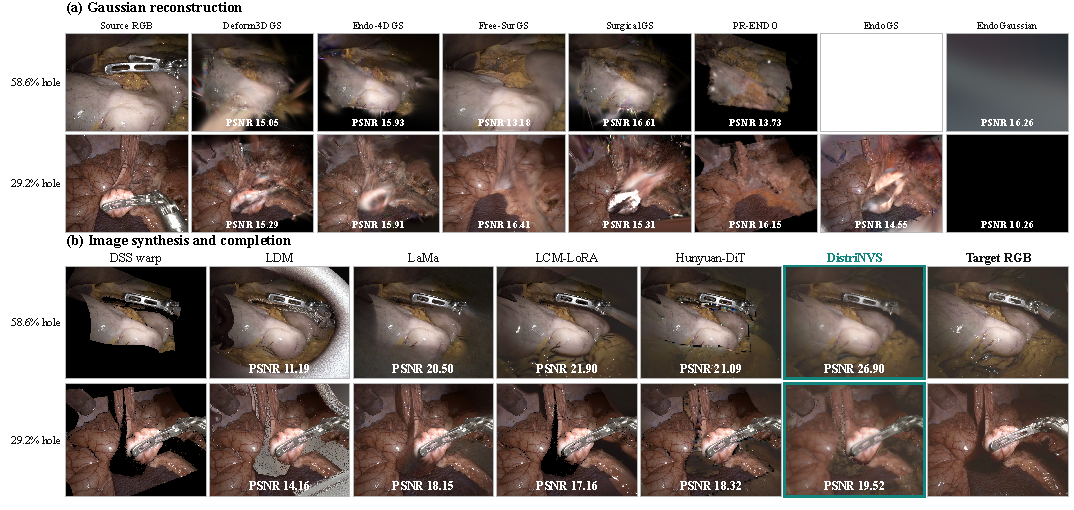
\includegraphics[width=\textwidth]{figures/table_comparisons/table1_qualitative_comparison.pdf}
\caption{Qualitative in-domain comparison on iMED\_NVS. (a) Gaussian reconstruction
from source RGB. (b) Image completion from the DSS warp. White labels report
full image PSNR (dB). In the second scene, residual tool misalignment may arise
from errors in the camera pose provided by the dataset.}
\label{fig:iMED_NVS-qualitative}
\vspace{-0.2cm}
\end{figure*}



\label{sec:implementation}
\begin{table}[t]
\centering
\caption{Full image quantitative comparison on the iMED\_NVS test set
($N=1{,}392$).}
\label{tab:validation-comparison}
\scriptsize
\setlength{\tabcolsep}{0pt}
\begin{tabularx}{\columnwidth}{@{}l*{3}{>{\centering\arraybackslash}X}@{}}
\toprule
Method & PSNR $\uparrow$ & SSIM $\uparrow$ & LPIPS $\downarrow$ \\
\midrule
Deform3DGS~\cite{yang2024deform3dgs} & $15.83\pm1.87$ & $0.33\pm0.06$ & $0.48\pm0.10$ \\
Endo-4DGS~\cite{huang2024endo4dgs} & $16.78\pm1.65$ & $0.36\pm0.04$ & $0.46\pm0.08$ \\
Free-SurGS~\cite{guo2024freesurgs} & $17.09\pm2.14$ & $\underline{0.43\pm0.07}$ & $0.51\pm0.07$ \\
SurgicalGS~\cite{chen2025surgicalgs} & $17.79\pm1.95$ & $0.38\pm0.07$ & $0.46\pm0.07$ \\
PR-ENDO~\cite{kaleta2025prendo} & $15.79\pm1.27$ & $0.31\pm0.07$ & $0.55\pm0.07$ \\
EndoGS~\cite{zhu2024endogs} & $12.52\pm6.22$ & $0.38\pm0.06$ & $0.66\pm0.20$ \\
EndoGaussian~\cite{liu2025endogaussian} & $14.38\pm4.26$ & $0.37\pm0.24$ & $0.77\pm0.12$ \\
LDM~\cite{rombach2022ldm} & $17.18\pm2.83$ & $0.34\pm0.06$ & $0.44\pm0.08$ \\
LaMa~\cite{suvorov2022lama} & $19.48\pm1.44$ & $0.43\pm0.11$ & $\mathbf{0.35\pm0.06}$ \\
LCM-LoRA~\cite{luo2023lcmlora} & $19.47\pm1.73$ & $0.42\pm0.12$ & $0.39\pm0.04$ \\
Hunyuan-DiT~\cite{li2024hunyuandit} & $\underline{19.52\pm1.51}$ & $0.42\pm0.12$ & $\underline{0.38\pm0.04}$ \\
\midrule
\rowcolor{gray!15} DistriNVS (SF) & $\mathbf{22.95\pm2.33}$ & $\mathbf{0.59\pm0.11}$ & $0.40\pm0.05$ \\
\bottomrule
\end{tabularx}
% \vspace{-0.4cm}
\end{table}




\begin{table}[t]
\centering
\caption{Unobserved region quantitative comparison on the iMED\_NVS test set
($N=1{,}392$).}
\label{tab:validation-comparison-hole}
\scriptsize
\setlength{\tabcolsep}{0pt}
\begin{tabularx}{\columnwidth}{@{}l*{3}{>{\centering\arraybackslash}X}@{}}
\toprule
Method & H-PSNR $\uparrow$ & H-SSIM $\uparrow$ & H-LPIPS $\downarrow$ \\
\midrule
Deform3DGS~\cite{yang2024deform3dgs} & $14.01\pm1.81$ & $0.31\pm0.07$ & $0.63\pm0.06$ \\
Endo-4DGS~\cite{huang2024endo4dgs} & $15.79\pm1.85$ & $0.42\pm0.14$ & $0.60\pm0.06$ \\
Free-SurGS~\cite{guo2024freesurgs} & $17.86\pm2.88$ & $0.56\pm0.05$ & $0.56\pm0.06$ \\
SurgicalGS~\cite{chen2025surgicalgs} & $17.63\pm2.87$ & $0.47\pm0.16$ & $0.59\pm0.06$ \\
PR-ENDO~\cite{kaleta2025prendo} & $11.92\pm1.71$ & $0.10\pm0.06$ & $0.74\pm0.08$ \\
EndoGS~\cite{zhu2024endogs} & $12.52\pm6.68$ & $0.49\pm0.12$ & $0.74\pm0.17$ \\
EndoGaussian~\cite{liu2025endogaussian} & $15.86\pm3.60$ & $0.48\pm0.31$ & $0.69\pm0.09$ \\
LDM~\cite{rombach2022ldm} & $14.90\pm3.48$ & $0.37\pm0.11$ & $0.64\pm0.13$ \\
LaMa~\cite{suvorov2022lama} & $21.40\pm2.32$ & $0.63\pm0.05$ & $0.42\pm0.08$ \\
LCM-LoRA~\cite{luo2023lcmlora} & $\underline{22.53\pm2.23}$ & $\underline{0.70\pm0.06}$ & $\underline{0.42\pm0.04}$ \\
Hunyuan-DiT~\cite{li2024hunyuandit} & $20.87\pm2.07$ & $0.64\pm0.08$ & $0.49\pm0.03$ \\
\midrule
\rowcolor{gray!15} DistriNVS (SF) & $\mathbf{27.95\pm2.91}$ & $\mathbf{0.80\pm0.07}$ & $\mathbf{0.41\pm0.05}$ \\
\bottomrule
\end{tabularx}
% \vspace{-0.4cm}
\end{table}



\subsection{Learning Objectives}

\textbf{Regional reconstruction.}
During training, target RGB $\I_t$ and target depth 
$\D_t\in\R_+^{1\times H\times W}$ provide supervision.
A tissue-valid mask $\M_t^{\rm tis}\in\{0,1\}^{1\times H\times W}$ excludes
annotated instruments when available. We define the predicted unreliable-region
mask as $\M^{\rm hole}=1-\M^{\rm rel}$, where
$\M^{\rm hole}\in\{0,1\}^{1\times H\times W}$. The unreliable, trusted, and
transition tissue masks are defined as
$\M_u=\M^{\rm hole}\cap \M_t^{\rm tis}$,
$\M_v=\M^{\rm rel}\cap \M_t^{\rm tis}$, and
$\M_b=\operatorname{Band}(\M^{\rm hole})\cap \M_t^{\rm tis}$, respectively; all
three lie in $\{0,1\}^{1\times H\times W}$. The
regional reconstruction loss
$\mathcal L_{\rm rec}(\widehat\I_t,\I_t;\M_u,\M_v,\M_b)$ applies robust
Charbonnier RGB penalties to these regions and a gradient penalty on
$\M_u\cup \M_b$~\cite{charbonnier1994two}.

\textbf{Depth supervision.}
The depth loss $\mathcal L_{\rm depth}$ is defined over
$(\mu,\sigma,\widehat\D_t;\D_s^{\rm gt},\M_s^{\rm gt},\D_t,\M_t^D)$, where
$\D_s^{\rm gt}\in\R_+^{1\times H\times W}$ and
$\M_s^{\rm gt},\M_t^D\in\{0,1\}^{1\times H\times W}$. It combines a Laplace
negative log-likelihood over the originally valid source samples with a
relative target depth error evaluated over $\M_t^D$ when target depth is
available~\cite{kendall2017uncertainties}.

\textbf{Cycle consistency and routing.}
For \emph{RGB-D-guided reprojection cycle consistency (RCC)}, the predicted RGB-D
is splatted through the inverse calibration to obtain backward-rendered RGB
$\I_s^{\rm back}\in[0,1]^{3\times H\times W}$. The cycle loss is
\begin{equation}
\mathcal L_{\rm RCC}
=\left\langle
\rho_\epsilon\!\left(\I_s^{\rm back}-\I_s\right)
\right\rangle_{\M_s^{\rm cyc}},
\label{eq:rcc-loss}
\end{equation}
where $\rho_\epsilon(x)=\sqrt{x^2+\epsilon^2}$ is the Charbonnier penalty,
$\epsilon=10^{-3}$, and $\langle\cdot\rangle_{\M_s^{\rm cyc}}$ denotes
averaging over valid cycle pixels identified by
$\M_s^{\rm cyc}\in\{0,1\}^{1\times H\times W}$~\cite{charbonnier1994two}.
Risk modulates the backward splat, but no depth cycle loss is imposed.
The routing loss uses binary cross-entropy
between the pre-sigmoid synthesis logits and a detached binary target derived
from $(S,V,\mathcal H)$.

\textbf{Uncertainty supervision and total objective.}
The \emph{uncertainty loss (UL)} trains the predicted risk as an error scale
within the unreliable regions defined by $\M_u$. Let
$\mathbf E$ be the channel-mean absolute RGB error map and $\mathbf s$ the
positive scale map obtained from $\U_t$ through a bounded affine transform. We use
\( \mathcal L_{\rm UL}
 =\left\langle \mathbf E/\mathbf s+\log \mathbf s\right\rangle_{\M_u}.\)
The complete objective groups these terms as
\begin{equation}
 \mathcal L=\mathcal L_{\rm rec}+\lambda_d\mathcal L_{\rm depth}
 +\lambda_c\mathcal L_{\rm RCC}+\lambda_r\mathcal L_{\rm router}
 +\lambda_u\mathcal L_{\rm UL},
\label{eq:total-loss}
\end{equation}
where $\lambda_d,\lambda_c,\lambda_r,\lambda_u\in\R_+$ are weights that
balance the depth, cycle-consistency, routing, and uncertainty terms,
respectively.

% At inference, the predictor consumes only source RGB-D, camera calibration,
% and relative pose, and ends at the fused predictions in
% Eqs.~\eqref{eq:expert-fusion-rgb} and~\eqref{eq:expert-fusion-depth}. Target
% RGB-D and instrument masks are used only
% for supervision or evaluation; the backward-cycle branch and deterministic
% image repair are disabled. The method assumes known
% zero-skew pinhole intrinsics, a rigid inter-endoscope transform, and an
% axis-aligned approximation to projected uncertainty; these assumptions delimit
% its present scope.

% During training, target RGB $\I_t\in[0,1]^{3\times H\times W}$ and target depth 
% $\D_t\in\R_+^{1\times H\times W}$ provide supervision.
% A tissue-valid mask $M_t^{\rm tis}\in\{0,1\}^{1\times H\times W}$ excludes
% annotated instruments when available. A regional reconstruction objective
% $\mathcal L_{\rm rec}$ combines robust RGB and gradient agreement across trusted,
% unreliable, and transition regions. These regions are determined by the
% reliability masks. A depth objective
% $\mathcal L_{\rm depth}$ combines a Laplace likelihood for the predicted source
% depth distribution with relative target-depth supervision when target depth is
% available.
% For \emph{RGB-D-guided reprojection cycle consistency (RCC)}, the predicted
% RGB-D is splatted back through the inverse calibrated transform and the
% backward-rendered RGB is compared with the valid source image. Risk modulates
% the backward splat, but no depth-cycle loss is imposed. The routing loss
% $\mathcal L_{\rm router}$ uses binary cross-entropy against a detached
% reliability target derived from DSS support, variance, and collision ambiguity.
% The \emph{uncertainty loss (UL)} trains risk as an error scale on the
% unreliable tissue mask $M_u\in\{0,1\}^{1\times H\times W}$. For pixel
% $p\in\Omega_t$, let $e_p\in\R_+$ be the channel-mean absolute RGB error and
% $s_p\in\R_+$ the positive scale obtained from $\U_t(p)$ through a bounded
% affine map. We use
% \begin{equation}
%  \mathcal L_{\rm UL}
%  =\left\langle e_p/s_p+\log s_p\right\rangle_{M_u}.
% \label{eq:risk-loss}
% \end{equation}

% The complete objective groups these terms as
% \begin{equation}
%  \mathcal L=\mathcal L_{\rm rec}+\lambda_d\mathcal L_{\rm depth}
%  +\lambda_c\mathcal L_{\rm RCC}+\lambda_r\mathcal L_{\rm router}
%  +\lambda_u\mathcal L_{\rm UL},
% \label{eq:total-loss}
% \end{equation}
% where $\lambda_d,\lambda_c,\lambda_r,\lambda_u\in\R_+$ are weights that
% balance geometry, cycle, routing, and uncertainty supervision, respectively.


\begin{figure*}[t]
\centering
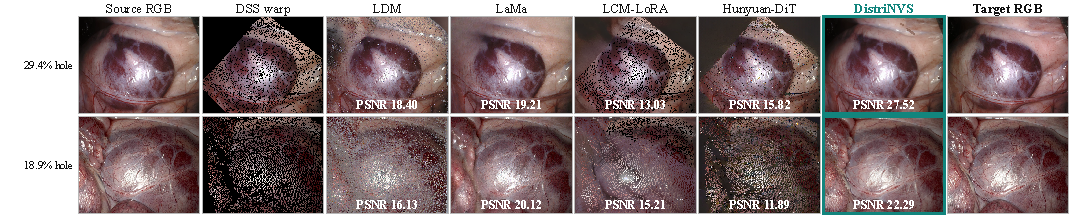
\includegraphics[width=\textwidth]{figures/table_comparisons/table2_zeroshot_qualitative_comparison.pdf}
\caption{Qualitative zero-shot comparison on SCARED dataset without adaptation
to the target domain. All completion baselines use the same DSS warp and
unsupported region mask. White labels report full image PSNR (dB). Hole
percentages denote the fraction of target pixels without raw DSS support.}
\label{fig:SCARED-qualitative}
\vspace{-0.2cm}
\end{figure*}




\section{Experiments}
\label{sec:experiments}

\subsection{Experimental Setup}

\textbf{Datasets.}
iMED\_NVS contains 20 scenes and is split at the scene level into 13 training scenes 
with 2561 synchronized pairs and 7 test scenes with 1392
pairs~\cite{imed2026}. 
Datasets~8 and 9 of SCARED~\cite{allan2021stereo} are used for zero-shot
evaluation. 
Each synchronized pair comprises a right camera RGB-D source and a left camera RGB target; 
DSS uses their intrinsics and calibrated relative camera pose.
We partition each sequence into temporal windows of 10 frames and select the
frame nearest to each window center while maintaining a separation of at least
five frames. This protocol yields 275 synchronized test pairs.

\textbf{Comparison Methods.}
We compare against seven endoscopic Gaussian reconstruction methods
~\cite{yang2024deform3dgs,huang2024endo4dgs,guo2024freesurgs,chen2025surgicalgs,kaleta2025prendo,zhu2024endogs,liu2025endogaussian}
and four feedforward completion systems: LDM, LaMa, LCM-LoRA, and
Hunyuan-DiT~\cite{rombach2022ldm,suvorov2022lama,luo2023lcmlora,li2024hunyuandit}. Every
prediction is evaluated at the same resolution on the same target frames. 
% We use the fine-tuned Hunyuan-DiT with the fixed
% 100-step DDPM protocol.


\textbf{Evaluation Metrics.}
We report PSNR~\cite{huynhthu2008psnr}, SSIM~\cite{wang2004ssim}, and LPIPS~\cite{zhang2018lpips}.
H-prefixed metrics are evaluated
on the canonical raw DSS hole intersected with non-tool tissue support on iMED\_NVS.
All SCARED pixels are evaluated because target tool masks are unavailable.
Latency is measured at batch size one on an
RTX~4090.
% , excluding loading, decoding, evaluation, and disk IO.
In evaluation, degenerate predictions are retained,
and all predictions are evaluated \textbf{without} postprocessing.
% The tables report frame-wise means and sample standard deviations.


\textbf{Implementation.}
Images are processed at spatial resolution $H\times W=512\times640$. DSS uses
the three Gaussian-weighted hypotheses described in Sec.~\ref{sec:method}, with
$(a_j)=(0.2741,0.4518,0.2741)$, $b=b_n=0.75$ pixels, and
$\tau_z=2$ mm. The routing prior weights are
$(\lambda_\kappa,\lambda_V,\lambda_H)=(0.65,0.20,0.15)$, 
with \(\epsilon=10^{-4}\) for clipping \(g^0\) before the logit transform.
The reliability encoder
transports 16 feature channels. The synthesis expert has four resolutions and
base width 32, and the complete network contains $5.79$\,M trainable
parameters. We optimize for $10^{4}$ epochs using AdamW with a learning rate of
$2\times10^{-4}$, weight decay $10^{-4}$, and effective batch size 12. The loss
weights are $(\lambda_d,\lambda_c,\lambda_r,\lambda_u)=(0.2,0.2,0.1,0.1)$.
Training
is performed on 4 NVIDIA RTX~4090 GPUs using BF16 mixed precision and seed
6666. Renderer, routing, mask, and loss constants are fixed across corresponding
configurations.

\subsection{In-Domain Comparison}

Tabs.~\ref{tab:validation-comparison} and
\ref{tab:validation-comparison-hole} compare all methods on the same 1392
iMED\_NVS frames using shared tissue and hole masks.
The Gaussian systems use dataset depth and serve as reconstruction references,
whereas DistriNVS is evaluated by its direct SF output.
% Bold and underlining mark the best and second-best means. 
On the iMED\_NVS test set, DistriNVS achieved the highest PSNR, SSIM, and
H-PSNR while remaining competitive in LPIPS. Fig.~\ref{fig:iMED_NVS-qualitative}
presents the corresponding qualitative evidence. Its examples are the 100th
retained pair from each of the lexicographically first and last test scenes, a
rule fixed before prediction inspection.
% Fig.~\ref{fig:hole-ratio} stratifies reconstruction quality by the fraction of
% target tissue unobserved by the source view. DistriNVS achieves the highest PSNR
% and lowest LPIPS in the largest-hole regime, indicating greater robustness to substantial
% target-only content.
We observe in Fig.~\ref{fig:iMED_NVS-qualitative} that the diffusion-based LCM-LoRA achieves the most accurate reconstruction in the shadowed regions.
Fig.~\ref{fig:hole-ratio} stratifies reconstruction quality by the fraction of
target tissue unobserved from the source view, termed the \emph{unobserved
ratio}. DistriNVS achieves the highest PSNR across all unobserved ratio ranges
and the lowest LPIPS in the largest missing regime, indicating greater
robustness under larger displacements between views and reduced overlap.





\begin{figure}[t]
\centering
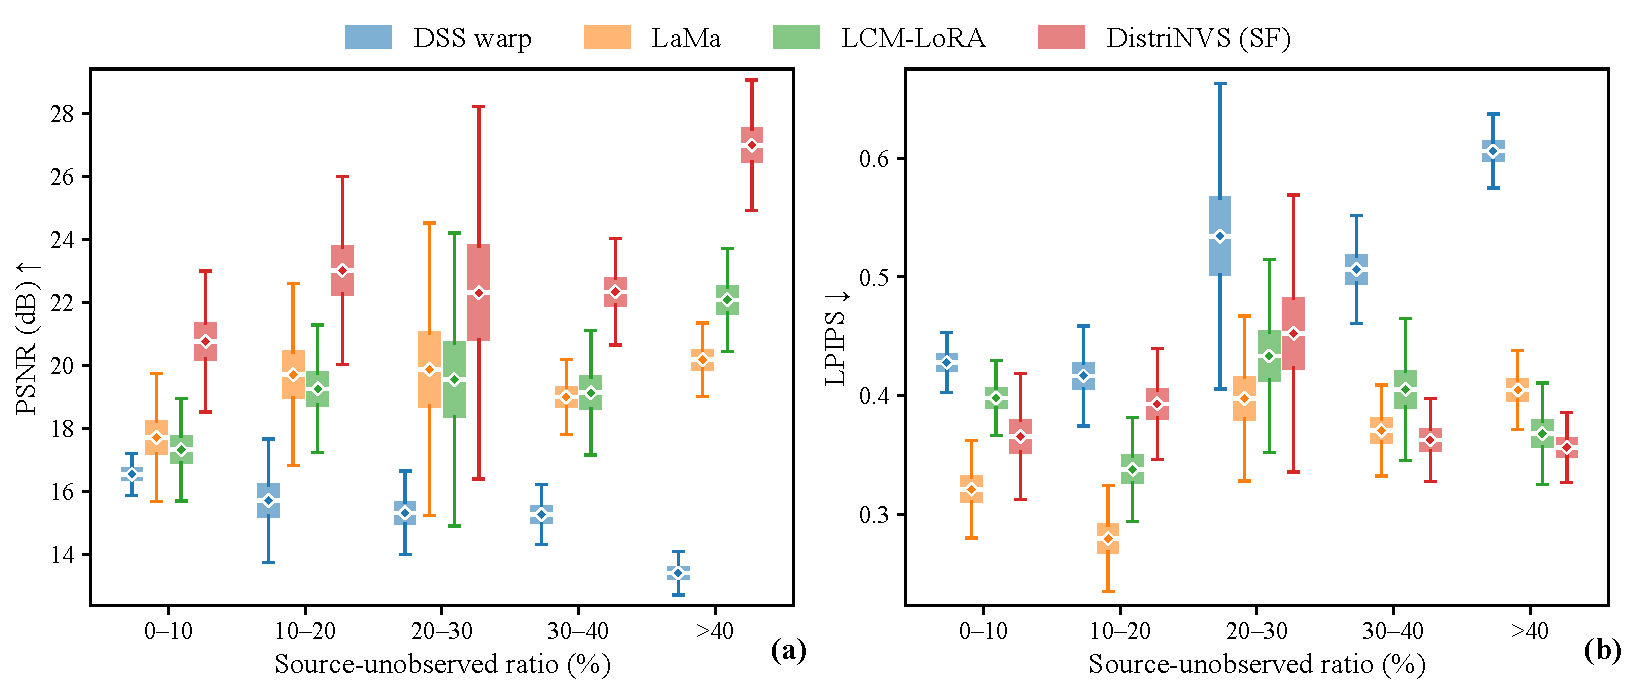
\includegraphics[width=\columnwidth]{figures/hole_ratio/hole_ratio_boxplot.pdf}
\caption{Performance stratified by the unobserved ratio on the iMED\_NVS test
set. Curves and shaded regions show the frame-wise mean and sample standard
deviation, respectively, for (a) PSNR and (b) LPIPS.}
\label{fig:hole-ratio}
\vspace{-0.2cm}
\end{figure}




\subsection{Zero-Shot Comparison}

We compare the five feedforward methods on the SCARED
dataset, without SCARED adaptation.
Bold and underlining in Tab.~\ref{tab:zeroshot-breakdown} mark the best and
second-best unrounded means.
On SCARED, DistriNVS achieved the highest PSNR and SSIM, the lowest LPIPS, and the
second-highest H-PSNR. It also had the second lowest latency, while
LaMa achieved the highest H-PSNR and the lowest latency. 
% The reported
% DistriNVS latency includes depth reliability estimation, DSS, routing, both
% experts, and output composition.
The slower inference of DistriNVS is partly due to the computational cost of DSS, 
whose distributional projection and aggregation operations add 
overhead beyond the synthesis network itself.
Fig.~\ref{fig:SCARED-qualitative} shows the qualitative results of the zero-shot comparison on the SCARED datasets.

\begin{table}[t]
\centering
\caption{Zero-shot comparison on SCARED Datasets~8 and 9 ($N=275$).}
% Baselines include LDM~\cite{rombach2022ldm}, LaMa~\cite{suvorov2022lama}, LCM-LoRA~\cite{luo2023lcmlora}, and Hunyuan-DiT~\cite{li2024hunyuandit}.}
\label{tab:zeroshot-breakdown}
\fontsize{6pt}{7pt}\selectfont
\setlength{\tabcolsep}{0pt}

\begin{tabularx}{\columnwidth}{@{}l*{5}{>{\centering\arraybackslash}X}@{}}
\toprule
Method
& PSNR $\uparrow$
& SSIM $\uparrow$
& LPIPS $\downarrow$
& H-PSNR $\uparrow$
& Latency (s) $\downarrow$ \\
\midrule
LDM
& $17.44{\pm}1.86$
& $0.33{\pm}0.14$
& $0.81{\pm}0.17$
& $12.54{\pm}2.44$
& $2.57{\pm}0.15$ \\
LaMa
& $\underline{22.72{\pm}2.10}$
& $\underline{0.63{\pm}0.14}$
& $\underline{0.32{\pm}0.07}$
& $\mathbf{21.43{\pm}2.71}$
& $\mathbf{0.04{\pm}0.00}$ \\
LCM-LoRA
& $14.26{\pm}0.94$
& $0.22{\pm}0.04$
& $1.00{\pm}0.08$
& $14.23{\pm}2.61$
& $0.40{\pm}0.04$ \\
Hunyuan-DiT
& $15.79{\pm}2.43$
& $0.31{\pm}0.12$
& $0.85{\pm}0.15$
& $13.24{\pm}3.21$
& $13.04{\pm}0.07$ \\
\midrule
\rowcolor{gray!15} DistriNVS
& $\mathbf{23.47{\pm}2.01}$
& $\mathbf{0.66{\pm}0.12}$
& $\mathbf{0.23{\pm}0.04}$
& $\underline{21.11{\pm}2.93}$
& $\underline{0.08{\pm}0.01}$ \\
\bottomrule
\end{tabularx}
% \vspace{-0.2cm}
\end{table}




\subsection{Ablation Study}

Tab.~\ref{tab:ablation} presents ablation results on the iMED\_NVS test set.
The primary model uses SF, whereas the six component
variants retain legacy HC.
SF achieved the strongest overall reconstruction in Tab.~\ref{tab:ablation}.
Within the HC mode, removing DD causes the clearest joint degradation,
whereas DC, OF, PGR, RCC, and UL show smaller or region-dependent changes.
% Because SF and HC are trained separately, the HC variants should not be read
% as direct removals from the primary SF model.



% =========================
% Table
% =========================
\begin{table}[t]
\centering
\caption{Ablation study on the iMED\_NVS test set
($N=1{,}392$).}
\label{tab:ablation}
\scriptsize
\setlength{\tabcolsep}{0pt}
\begin{tabular*}{\columnwidth}
{@{}l@{\extracolsep{\fill}}rrrr@{}}
\toprule
Variant
& PSNR $\uparrow$
& SSIM $\uparrow$
& H-PSNR $\uparrow$
& H-SSIM $\uparrow$ \\
\midrule
\rowcolor{gray!15}
\multicolumn{5}{c}{
    \rule{0pt}{2.3ex}
    \textbf{Primary output rule and legacy reference}
} \\
DistriNVS (SF)
& $\mathbf{22.95\pm2.33}$
& $\mathbf{0.59\pm0.11}$
& $\mathbf{27.95\pm2.91}$
& $\mathbf{0.80\pm0.07}$ \\
DistriNVS (HC)
& $\underline{20.77\pm1.91}$
& $\underline{0.49\pm0.13}$
& $27.56\pm2.73$
& $0.78\pm0.07$ \\
\addlinespace
\rowcolor{gray!15}
\multicolumn{5}{c}{
    \rule{0pt}{2.3ex}
    \textbf{Component variants under legacy HC}
} \\
w/o DC
& $20.68\pm1.89$
& $0.49\pm0.13$
& $\underline{27.76\pm2.48}$
& $\underline{0.79\pm0.06}$ \\
w/o DD
& $20.67\pm1.91$
& $0.48\pm0.13$
& $27.19\pm2.74$
& $0.77\pm0.07$ \\
w/o OF
& $20.65\pm1.92$
& $0.48\pm0.13$
& $27.73\pm2.71$
& $0.78\pm0.06$ \\
w/o PGR
& $20.75\pm1.89$
& $0.49\pm0.13$
& $27.41\pm2.72$
& $0.77\pm0.07$ \\
w/o RCC
& $20.72\pm1.91$
& $0.49\pm0.13$
& $27.41\pm2.73$
& $0.78\pm0.07$ \\
w/o UL
& $20.70\pm1.89$
& $0.48\pm0.13$
& $27.02\pm2.60$
& $0.77\pm0.07$ \\
\bottomrule
\end{tabular*}
% \vspace{-0.4cm}
\end{table}



% \section{Discussion}
% \label{sec:discussion}

% Our ablation indicates that the output rule has the largest effect, while DD
% provides the most consistent component-level benefit within the HC family.
% We observe smaller or region-dependent effects from the remaining components.
% This pattern is consistent with HC preserving residual transport error, whereas
% SF permits bounded appearance correction. Because SF and HC differ during both
% training and inference, their comparison does not isolate the output operation
% alone. Our ablation also uses a single seed, and the component variants are
% trained under HC; their interactions with the primary SF model therefore remain
% untested. We further note that the fixed SCARED benchmark is frame-weighted
% with an uneven sequence distribution, although all methods use the same pairs
% without evaluator-side repair.

\subsection{Performance Analysis}

We observe a remaining gap to LaMa on several specific metrics, which may stem
from differences in model capacity and training objectives. LaMa uses approximately 51M parameters and combines global Fourier processing with adversarial, feature matching, and perceptual objectives tailored to image inpainting.
By contrast, our model uses only 5.79M
parameters while allocating capacity to geometry transport, reliability
estimation, routing, RGB-D prediction, and uncertainty modeling. Endoscopic
tissue often exhibits smooth color variation and texture dominated by low
frequencies, which may favor LaMa's larger inpainting network. This difference may
explain its lower LPIPS on iMED\_NVS and its H-PSNR advantage on SCARED.
Our results nevertheless show that DistriNVS achieves better zero-shot PSNR,
SSIM, and LPIPS on SCARED while using about one ninth as many parameters.
% Future work will explore increasing the capacity of our synthesis expert and 
% introducing perceptual or adversarial supervision
% while retaining the geometry-derived
% reliability constraints that distinguish transported evidence from synthesized
% content.

\section{Conclusion}
\label{sec:conclusion}

In this paper, we introduce DistriNVS, a reliability-aware framework for
cross-endoscope novel view synthesis that separates geometry-supported
transport from target-only synthesis. DistriNVS combines distributional surface
splatting, which propagates depth uncertainty and estimates target view
reliability, with reliability-constrained expert fusion that preserves supported
evidence while completing unobserved regions. Extensive experiments on
iMED\_NVS and zero-shot SCARED show that DistriNVS outperforms Gaussian
reconstruction and image completion baselines, particularly when large target
regions are unobserved by the source view.

\balance
\bibliographystyle{IEEEtran}
\bibliography{references}

\end{document}
